\documentclass[UTF8,a4paper,12pt]{ctexart}

\usepackage{geometry}
\usepackage{array}
\usepackage{tabularx}
\usepackage{booktabs}
\usepackage{longtable}
\usepackage{enumitem}
\usepackage{xcolor}
\usepackage{listings}
\usepackage{graphicx}
\usepackage{hyperref}
\usepackage{fancyhdr}
\usepackage{float}

\geometry{left=2.6cm,right=2.6cm,top=2.5cm,bottom=2.5cm}
\setlength{\headheight}{15pt}
\setlist{nosep,leftmargin=2em}
\hypersetup{
  colorlinks=true,
  linkcolor=black,
  urlcolor=blue
}
\newcolumntype{Y}{>{\raggedright\arraybackslash}X}

\pagestyle{fancy}
\fancyhf{}
\lhead{软件测试作业二：GUI 测试}
\rhead{测试报告}
\cfoot{\thepage}

\lstset{
  basicstyle=\ttfamily\small,
  breaklines=true,
  frame=single,
  columns=fullflexible,
  backgroundcolor=\color{gray!8}
}

\begin{document}

\begin{center}
  {\LARGE\bfseries 测试报告}
\end{center}
\thispagestyle{empty}
\vspace{1em}
\tableofcontents
\newpage

\section{测试概述}

本次 GUI 自动化测试以 SauceDemo 电商网站为被测对象，围绕电商网站中常见的商品浏览、排序、详情查看、购物车、结算和移动端补充验证等事务开展测试。SauceDemo 页面结构清晰，业务流程完整，且包含按钮、输入框、表单、下拉框、链接、侧边栏、购物车标记等多种 Web 元素，适合作为课程作业中的 GUI 自动化测试对象。

测试采用 Selenium WebDriver 模拟用户在桌面浏览器中的真实操作，并使用 pytest 组织测试用例和执行结果。移动端部分采用 Appium、UiAutomator2 Driver 和 Android 模拟器中的 Chrome 浏览器执行，用于补充验证 SauceDemo 在真实移动端浏览器环境下的核心购物流程。报告围绕测试计划中确定的功能事务展开，记录测试设计、Web 元素覆盖、用例执行结果和测试结论。

被测网站：

\begin{lstlisting}
https://www.saucedemo.com/
\end{lstlisting}

测试账号：

\begin{lstlisting}
username: standard_user
password: secret_sauce
\end{lstlisting}

图 \ref{fig:homepage-comparison} 展示了 SauceDemo 在桌面端浏览器和 Android 模拟器 Chrome 中的商品列表首页。桌面端页面用于执行 TC01--TC07 的 Web UI 自动化测试，移动端页面用于执行 TC08 的 Appium 移动端 Web UI 综合验证。

\begin{figure}[H]
\centering
\begin{minipage}[c]{0.62\textwidth}
\centering
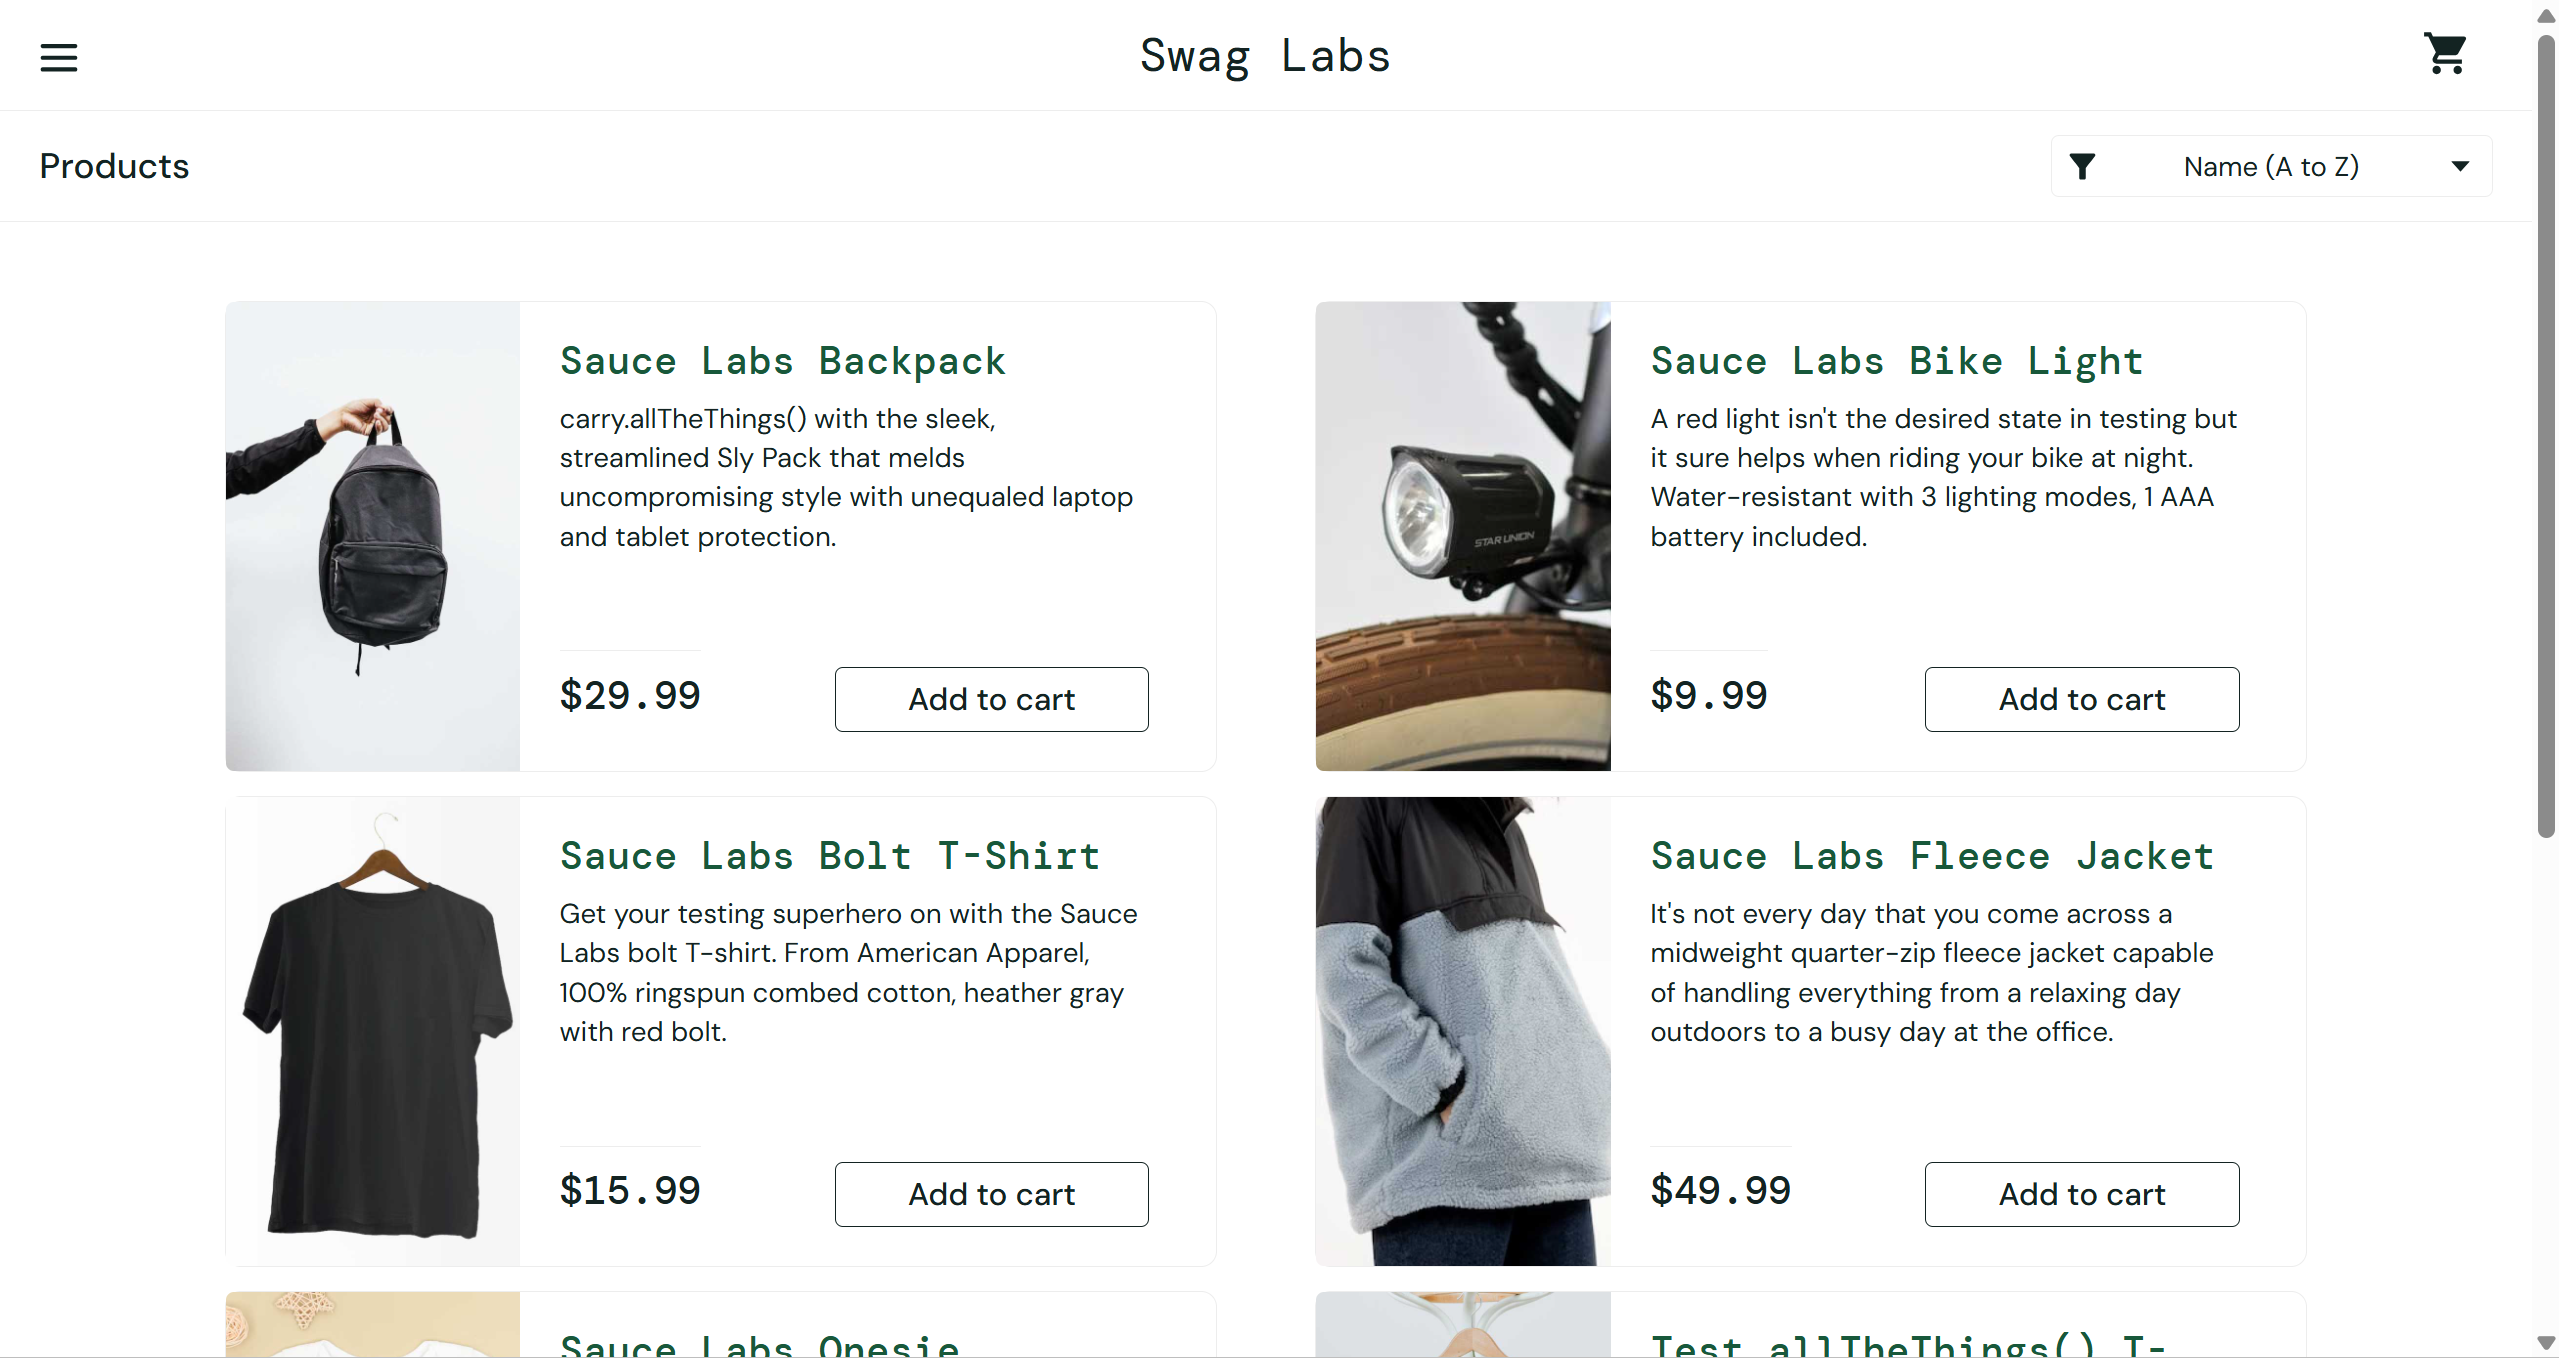
\includegraphics[width=\textwidth]{Figures/web_homepage_即商品列表.png}
{\small 桌面端商品列表页}
\end{minipage}
\hfill
\begin{minipage}[c]{0.28\textwidth}
\centering
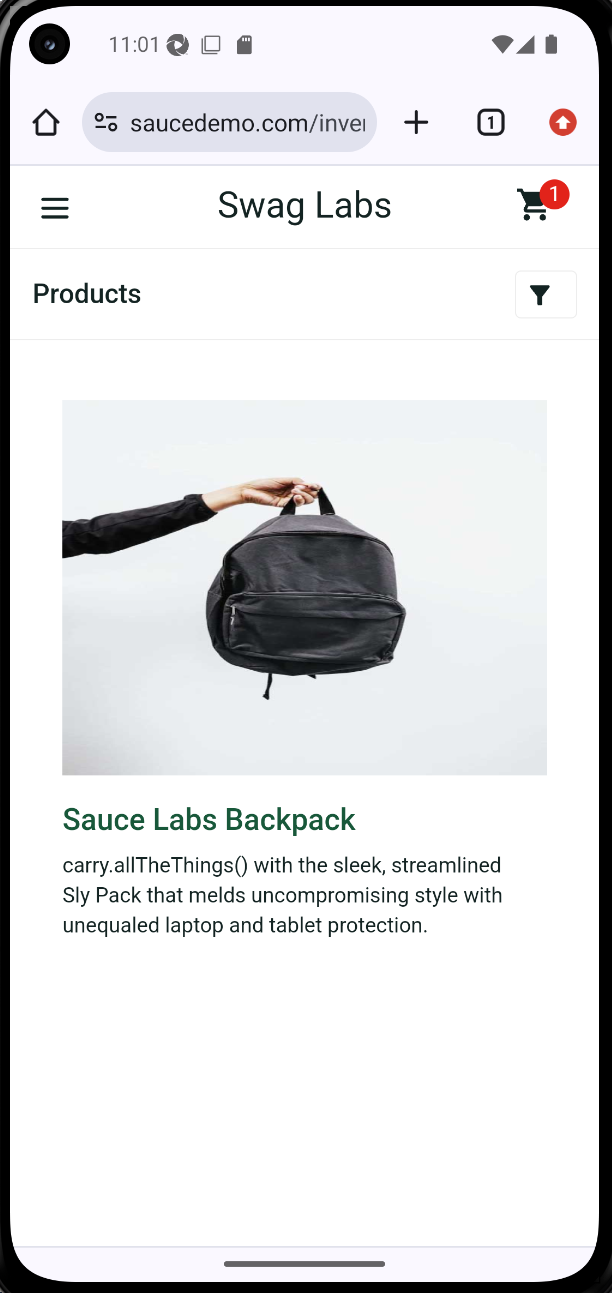
\includegraphics[width=\textwidth]{Figures/mobile_homepage_商品列表.png}
{\small 移动端商品列表页}
\end{minipage}
\caption{桌面端与移动端商品列表首页对比}
\label{fig:homepage-comparison}
\end{figure}

\section{测试范围}

本次测试覆盖 SauceDemo 的核心购物路径：

\begin{lstlisting}
登录页 -> 商品列表页 -> 商品详情页 -> 购物车页 -> 结算页 -> 订单完成页
\end{lstlisting}

整体测试事务包括登录后进入商品浏览流程、商品排序、查看商品详情、添加商品到购物车、购物车页面检查、结算与订单完成、侧边栏导航菜单和移动端 Web UI 综合验证。其中，TC01--TC07 为桌面端 Web 自动化测试，用于验证主要业务功能；TC08 为 Appium 移动端补充测试，用于在 Android Chrome 中验证登录、商品浏览、排序、页面滚动、商品详情、购物车、结算和订单完成等核心流程。

\section{测试环境与工具}

测试环境使用独立 conda 环境管理 Python 依赖，避免与本机其他课程项目或 Python 包版本产生冲突。桌面端测试代码采用 Page Object 思路封装页面元素和页面行为，将页面定位、页面操作和测试断言分离，使测试代码结构更清晰，也便于定位失败原因。移动端测试通过 Appium Server 连接 Android 模拟器，并驱动模拟器中的 Chrome 浏览器执行 Web UI 操作。

\begin{table}[H]
\centering
\caption{桌面端 Web UI 测试环境与工具}
\begin{tabularx}{\textwidth}{>{\bfseries}p{3.2cm}X}
\toprule
项目 & 内容 \\
\midrule
操作系统 & Windows \\
浏览器 & Google Chrome \\
编程语言 & Python 3.11 \\
Python 环境 & conda 环境：saucedemo-gui-test \\
自动化框架 & Selenium WebDriver \\
测试运行框架 & pytest \\
测试组织方式 & Page Object + pytest fixture \\
\bottomrule
\end{tabularx}
\end{table}

\begin{table}[H]
\centering
\caption{移动端 Web UI 测试环境与工具}
\begin{tabularx}{\textwidth}{>{\bfseries}p{3.2cm}X}
\toprule
项目 & 内容 \\
\midrule
移动端设备 & Android Studio 模拟器 \\
移动端浏览器 & Android Chrome \\
设备连接工具 & adb \\
Appium Server & Appium 2，监听地址 http://127.0.0.1:4723 \\
自动化驱动 & UiAutomator2 Driver \\
Python 客户端 & Appium-Python-Client \\
测试运行框架 & pytest \\
启动要求 & Android 模拟器保持运行，Appium Server 使用 appium --allow-insecure chromedriver\_autodownload 启动。 \\
\bottomrule
\end{tabularx}
\end{table}

\section{测试功能或事务设计}

测试功能设计以完整用户事务为单位，而不是单独罗列页面元素。登录操作不作为孤立功能统计，而是作为进入商品浏览流程的必要前置步骤；商品排序、商品详情、购物车、结算、导航和移动端抽测分别对应 SauceDemo 中不同层级的页面与交互。这样的设计既符合购物流程的真实使用顺序，也能够满足作业对 5 个及以上功能或事务、多页面跳转和多类 Web 元素覆盖的要求。

\begin{longtable}{p{1.5cm}p{4.5cm}p{8cm}}
\caption{测试功能或事务设计}\\
\toprule
编号 & 功能或事务 & 测试目标 \\
\midrule
\endfirsthead
\toprule
编号 & 功能或事务 & 测试目标 \\
\midrule
\endhead
TC01 & 登录后进入商品浏览流程 & 验证登录表单可用，使用标准账号登录后能够进入商品列表页，并检查商品页关键元素是否正常显示。 \\
TC02 & 商品排序 & 验证商品排序下拉框可见，排序选项完整，并检查名称升序、名称降序、价格升序、价格降序四种排序结果。 \\
TC03 & 查看商品详情 & 验证从商品列表页点击商品名称或图片后能够进入商品详情页，并检查商品名称、描述、价格、图片和返回入口。 \\
TC04 & 添加商品到购物车 & 验证商品能够从列表页或详情页加入购物车，并检查按钮状态和购物车 badge 数量变化。 \\
TC05 & 购物车页面检查 & 验证点击购物车入口后能够进入购物车页，并检查购物车中商品名称、价格、数量和结算入口。 \\
TC06 & 结算与订单完成 & 验证购物车商品能够进入结算流程，填写结算信息后完成订单，并检查订单完成提示。 \\
TC07 & 侧边栏导航菜单 & 验证商品列表页侧边栏菜单能够正常展开、显示导航项并关闭。 \\
TC08 & 移动端 Web UI 综合验证 & 使用 Appium 驱动 Android 模拟器 Chrome，验证移动端环境下核心购物流程是否可用。 \\
\bottomrule
\end{longtable}

\section{Web 元素覆盖情况}

根据作业要求，本次测试需要覆盖按钮、输入框、表单、下拉框、链接等必选 Web 元素，并至少覆盖一种可选元素。整体测试设计围绕 SauceDemo 的购物流程展开：商品列表页覆盖排序下拉框、商品详情入口和购物车入口；商品详情、购物车和结算流程覆盖商品链接、购物车 badge、结算表单和多个操作按钮；侧边栏导航和移动端抽测覆盖导航栏、触控点击和页面滑动等可选元素。登录页中的账号密码输入框、登录表单和 Login 按钮作为进入购物流程的必要入口进行基础检查，但不作为独立业务功能统计。

从整体覆盖角度看，测试对象能够满足多页面、多元素、多操作类型的 GUI 测试要求，元素覆盖与测试事务之间具有明确对应关系。

\begingroup
\small
\setlength{\tabcolsep}{2pt}
\begin{longtable}{p{2.4cm}p{8.6cm}@{\hspace{0.4cm}}p{3.6cm}}
\caption{Web 元素覆盖情况}\\
\toprule
元素类型 & SauceDemo 中的对应元素 & 对应用例 \\
\midrule
\endfirsthead
\toprule
元素类型 & SauceDemo 中的对应元素 & 对应用例 \\
\midrule
\endhead
按钮 & 登录按钮（Login）、加入购物车按钮（Add to cart）、移除按钮（Remove）、结算按钮（Checkout）、继续按钮（Continue）、完成按钮（Finish）、侧边栏关闭按钮 & TC01、TC04、TC05、TC06、TC07 \\
输入框 & 用户名输入框（username）、密码输入框（password）、姓名输入框（first name、last name）、邮政编码输入框（postal code） & TC01、TC06 \\
表单 & 登录表单、结算信息表单 & TC01、TC06 \\
下拉框 & 商品排序下拉框 & TC02 \\
链接 & 商品名称链接、商品图片链接、购物车链接、侧边栏菜单项 & TC03、TC05、TC07 \\
侧边栏/导航栏 & 左侧菜单按钮、全部商品（All Items）、关于页面（About）、退出登录（Logout）、重置应用状态（Reset App State） & TC07 \\
购物车数量标记 & 购物车图标旁显示的商品数量标记（badge） & TC04、TC05 \\
移动端触控/滑动 & Android Chrome 中的触控点击、页面滚动与元素定位 & TC08 \\
\bottomrule
\end{longtable}
\endgroup

\section{测试用例与执行结果}

测试用例按照“操作步骤可复现、检查点明确、结果可断言”的原则编写。自动化测试使用 Selenium 模拟真实浏览器操作，并通过 pytest 对页面跳转、元素显示状态、业务数据和交互结果进行断言。测试失败时会自动在 artifacts/screenshots 目录下保存截图，便于定位问题。

用例执行前需确认 conda 环境、Python 依赖和 Chrome 浏览器可用。执行过程中浏览器由测试 fixture 自动启动，测试结束后自动关闭浏览器实例。各测试事务的具体步骤、检查点和执行结果在以下小节中分别记录。

移动端 TC08 执行前还需额外确认 Android 模拟器已启动、adb 能识别设备，并使用 \verb|appium --allow-insecure chromedriver_autodownload| 启动 Appium Server。由于 Android Chrome 版本与 Chromedriver 需要匹配，测试过程中启用 Chromedriver 自动下载能力以保证 Appium 能够正常控制模拟器浏览器。

\subsection{TC01 登录后进入商品浏览流程}

TC01 用于验证用户能否通过标准账号进入商品浏览页面。该用例覆盖登录页表单填写、按钮点击、页面跳转和商品列表页加载结果，是整个购物流程自动化测试的入口用例。

\begin{table}[H]
\centering
\caption{TC01 测试结果}
\begin{tabularx}{\textwidth}{>{\bfseries}p{3cm}X}
\toprule
项目 & 内容 \\
\midrule
测试文件 & tests/test\_tc01\_login\_inventory.py \\
前置条件 & Chrome 浏览器可启动，网络可访问 SauceDemo，使用账号 standard\_user / secret\_sauce。 \\
测试步骤 & 打开登录页；检查登录表单、用户名输入框、密码输入框和 Login 按钮；输入账号密码并点击 Login；等待商品列表页加载。 \\
实际检查点 & URL 包含 /inventory.html；页面标题为 Products；商品数量为 6；商品名称数量为 6；排序下拉框可见；购物车入口可见。 \\
预期结果 & 登录成功并进入商品列表页，商品列表页关键元素正常显示。 \\
执行结果 & 通过。 \\
\bottomrule
\end{tabularx}
\end{table}

执行结果表明，标准账号能够正常登录，登录后页面能够稳定跳转至商品列表页；商品列表页中的标题、商品条目、排序下拉框和购物车入口均能被 Selenium 定位并通过断言检查。

\begin{figure}[H]
\centering
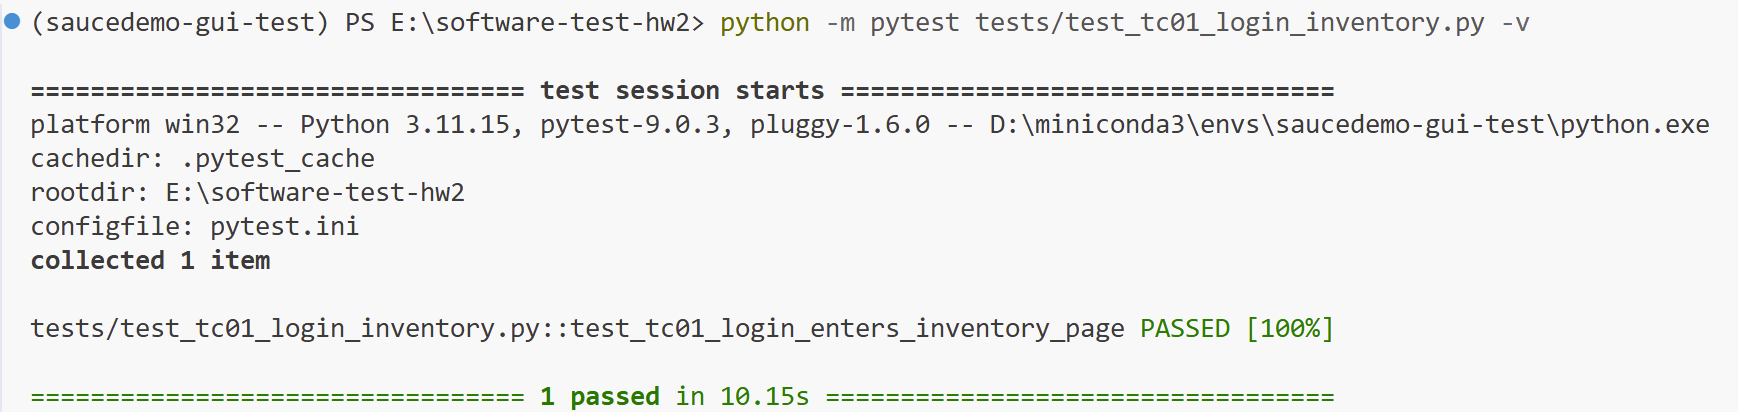
\includegraphics[width=0.92\textwidth]{Figures/TC01_result.png}
\caption{TC01 登录后进入商品浏览流程执行结果截图}
\end{figure}

\subsection{TC02 商品排序}

TC02 用于验证商品列表页排序下拉框的可用性。排序是商品浏览场景中的常见交互，本用例通过检查下拉框选项和排序后的商品顺序，确认该控件既能够被操作，也能够产生正确的页面结果。

\begin{table}[H]
\centering
\caption{TC02 测试结果}
\begin{tabularx}{\textwidth}{>{\bfseries}p{3cm}X}
\toprule
项目 & 内容 \\
\midrule
测试文件 & tests/test\_tc02\_product\_sorting.py \\
前置条件 & 已使用标准账号登录并进入商品列表页。 \\
测试步骤 & 检查排序下拉框可见；检查下拉框选项；依次选择 Name (Z to A)、Name (A to Z)、Price (low to high)、Price (high to low)。 \\
实际检查点 & 下拉框选项包含 4 项；商品名称降序结果正确；商品名称升序结果正确；价格升序结果正确；价格降序结果正确。 \\
预期结果 & 商品列表能够按照所选排序规则正确排列。 \\
执行结果 & 通过。 \\
\bottomrule
\end{tabularx}
\end{table}

执行结果表明，商品排序下拉框包含 4 个预期选项；选择不同排序规则后，商品名称和价格列表均能按照对应规则排列，说明排序控件和页面结果更新均符合预期。

\begin{figure}[H]
\centering
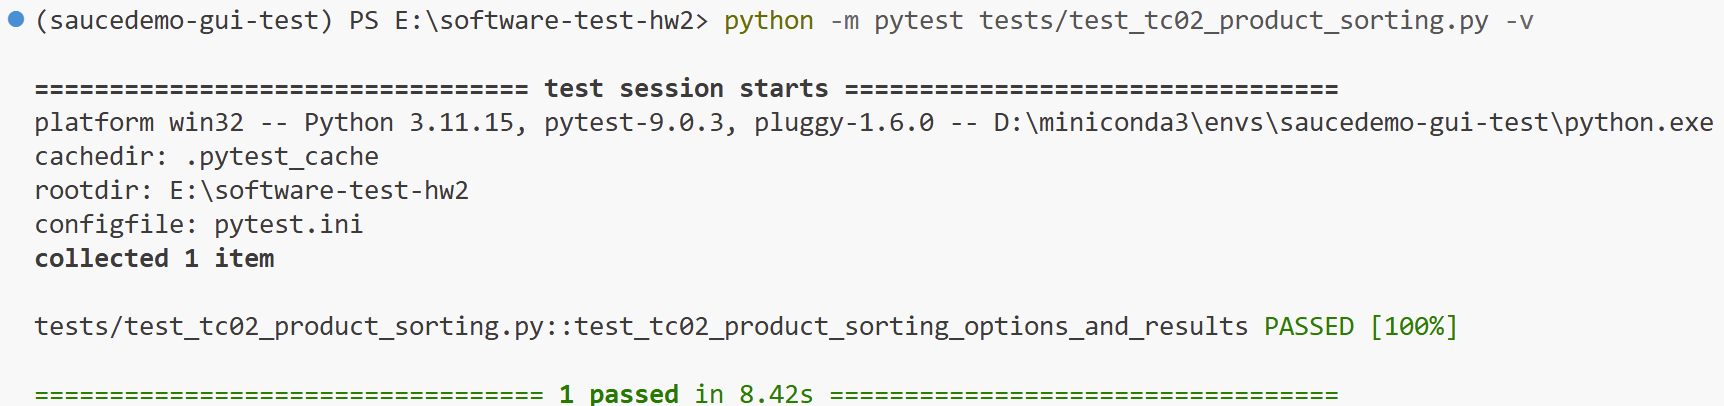
\includegraphics[width=0.92\textwidth]{Figures/TC02_result.png}
\caption{TC02 商品排序执行结果截图}
\end{figure}

\subsection{TC03 查看商品详情}

TC03 用于验证用户从商品列表页进入商品详情页的页面跳转和详情信息展示。该用例覆盖商品名称链接、商品详情页中的商品名称、描述、价格、图片、Add to cart 按钮以及 Back to products 返回入口。

\begin{table}[H]
\centering
\caption{TC03 测试结果}
\begin{tabularx}{\textwidth}{>{\bfseries}p{3cm}X}
\toprule
项目 & 内容 \\
\midrule
测试文件 & tests/test\_tc03\_product\_detail.py \\
前置条件 & 已使用标准账号登录并进入商品列表页。 \\
测试步骤 & 获取商品列表页中 Sauce Labs Backpack 的描述和价格；点击商品名称进入详情页；检查详情页 URL、商品名称、描述、价格、图片和 Add to cart 按钮；点击 Back to products 返回商品列表页。 \\
实际检查点 & URL 包含 /inventory-item.html；详情页商品名称为 Sauce Labs Backpack；商品描述和价格与列表页一致；商品图片可见；Add to cart 按钮可见；返回后页面标题为 Products。 \\
预期结果 & 能够正常进入商品详情页，详情页商品信息完整且与商品列表页一致，返回按钮可正常回到商品列表页。 \\
执行结果 & 通过。 \\
\bottomrule
\end{tabularx}
\end{table}

执行结果表明，商品详情页能够通过商品名称链接正常打开，商品标题、描述、价格和图片均显示正确，详情页返回商品列表页的操作也符合预期。

\begin{figure}[H]
\centering
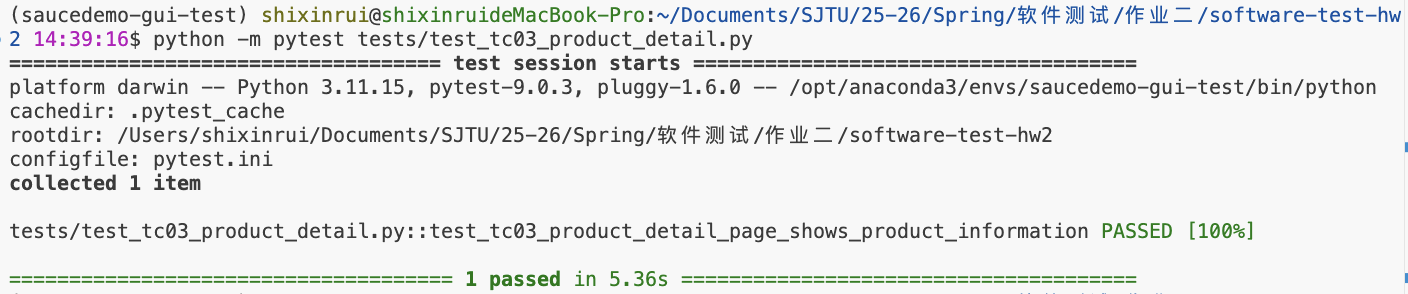
\includegraphics[width=0.92\textwidth]{Figures/TC03_result.png}
\caption{TC03 查看商品详情执行结果截图}
\end{figure}

\subsection{TC04 添加商品到购物车}

TC04 用于验证商品加入购物车后的页面状态变化。该用例分别从商品列表页和商品详情页执行 Add to cart 操作，检查按钮状态是否变为 Remove，并检查购物车 badge 数量是否随添加商品数量正确增加。

\begin{table}[H]
\centering
\caption{TC04 测试结果}
\begin{tabularx}{\textwidth}{>{\bfseries}p{3cm}X}
\toprule
项目 & 内容 \\
\midrule
测试文件 & tests/test\_tc04\_add\_to\_cart.py \\
前置条件 & 已使用标准账号登录并进入商品列表页，购物车初始为空。 \\
测试步骤 & 在商品列表页点击 Sauce Labs Backpack 的 Add to cart 按钮；检查按钮文本和购物车 badge；点击 Sauce Labs Bike Light 的商品名称链接进入商品详情页；在详情页点击 Add to cart；再次检查按钮文本和购物车 badge。 \\
实际检查点 & 第一个商品加入购物车后按钮文本变为 Remove，购物车 badge 显示 1；通过商品名称链接进入第二个商品详情页后，点击 Add to cart，按钮文本变为 Remove，购物车 badge 显示 2。 \\
预期结果 & 商品能够从列表页和详情页成功加入购物车，按钮状态和购物车数量标记能够正确反映购物车状态。 \\
执行结果 & 通过。 \\
\bottomrule
\end{tabularx}
\end{table}

执行结果表明，SauceDemo 的 Add to cart 按钮在列表页和详情页均可正常使用；商品加入购物车后按钮状态和购物车 badge 数量变化正确。

\begin{figure}[H]
\centering
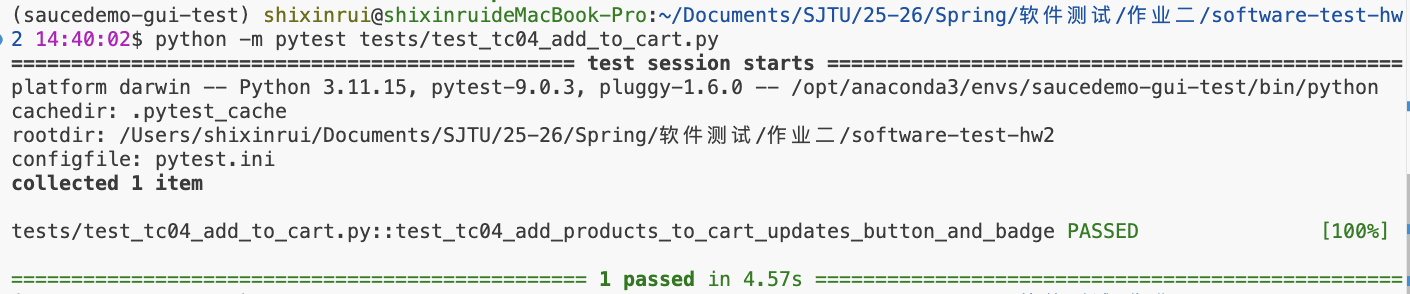
\includegraphics[width=0.92\textwidth]{Figures/TC04_result.png}
\caption{TC04 添加商品到购物车执行结果截图}
\end{figure}

\subsection{TC05 购物车页面检查}

TC05 用于验证已添加商品在购物车页面中的展示结果。该用例在商品加入购物车后进入购物车页，检查页面标题、商品名称、描述、价格、数量以及 Continue Shopping 和 Checkout 按钮。

\begin{table}[H]
\centering
\caption{TC05 测试结果}
\begin{tabularx}{\textwidth}{>{\bfseries}p{3cm}X}
\toprule
项目 & 内容 \\
\midrule
测试文件 & tests/test\_tc05\_cart\_page.py \\
前置条件 & 已使用标准账号登录并进入商品列表页。 \\
测试步骤 & 获取 Sauce Labs Backpack 在商品列表页中的描述和价格；点击该商品的 Add to cart；检查购物车 badge；点击购物车链接进入购物车页；检查购物车页面商品信息和操作按钮。 \\
实际检查点 & 商品加入购物车后 badge 显示 1；购物车页标题为 Your Cart；购物车商品条目数为 1；商品名称为 Sauce Labs Backpack；该商品数量字段为 1；商品描述和价格与列表页一致；Continue Shopping 和 Checkout 按钮可见。 \\
预期结果 & 购物车页面能够显示已添加商品，商品名称、描述、价格和数量正确，继续购物和结算入口正常显示。 \\
执行结果 & 通过。 \\
\bottomrule
\end{tabularx}
\end{table}

执行结果表明，购物车页面能够正确展示已添加商品，商品标题、描述、价格和数量与预期一致，Continue Shopping 和 Checkout 按钮均可被定位并正常显示。

\begin{figure}[H]
\centering
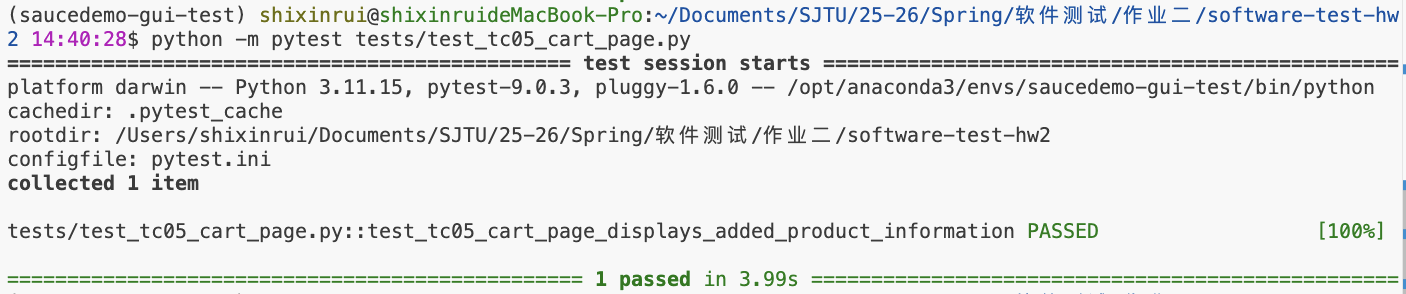
\includegraphics[width=0.92\textwidth]{Figures/TC05_result.png}
\caption{TC05 购物车页面检查执行结果截图}
\end{figure}

\subsection{TC06 结算与订单完成}

TC06 用于验证用户从购物车进入结算流程并完成订单的完整路径。该用例在已登录并添加商品的基础上，依次进入购物车页、结算信息页、订单确认页和订单完成页，检查结算表单输入框、Continue 按钮、Finish 按钮以及订单完成提示。

\begin{table}[H]
\centering
\caption{TC06 测试结果}
\begin{tabularx}{\textwidth}{>{\bfseries}p{3cm}X}
\toprule
项目 & 内容 \\
\midrule
测试文件 & tests/test\_tc06\_checkout.py \\
前置条件 & 已使用标准账号登录并进入商品列表页。 \\
测试步骤 & 获取 Sauce Labs Backpack 在商品列表页中的价格；点击该商品的 Add to cart；进入购物车页并点击 Checkout；在结算信息页填写 first name、last name 和 postal code；点击 Continue 进入订单确认页；检查确认页商品信息；点击 Finish 完成订单。 \\
实际检查点 & 结算信息页标题为 Checkout: Your Information；结算表单、first name 输入框、last name 输入框和 postal code 输入框可见；订单确认页标题为 Checkout: Overview；确认页商品条目数为 1；商品名称为 Sauce Labs Backpack；商品价格与列表页一致；Finish 按钮可见；订单完成页标题为 Checkout: Complete!；完成页显示 Thank you for your order! 和返回首页按钮。 \\
预期结果 & 用户能够从购物车正常进入结算流程，填写结算信息后进入订单确认页，并成功完成订单，页面显示订单完成提示。 \\
执行结果 & 通过。 \\
\bottomrule
\end{tabularx}
\end{table}

执行结果表明，SauceDemo 的结算流程能够从购物车页稳定跳转至结算信息页，结算表单中的姓名和邮政编码输入框能够正常填写；提交信息后订单确认页能够正确展示待结算商品及价格，点击 Finish 后能够进入订单完成页并显示订单完成提示。

\begin{figure}[H]
\centering
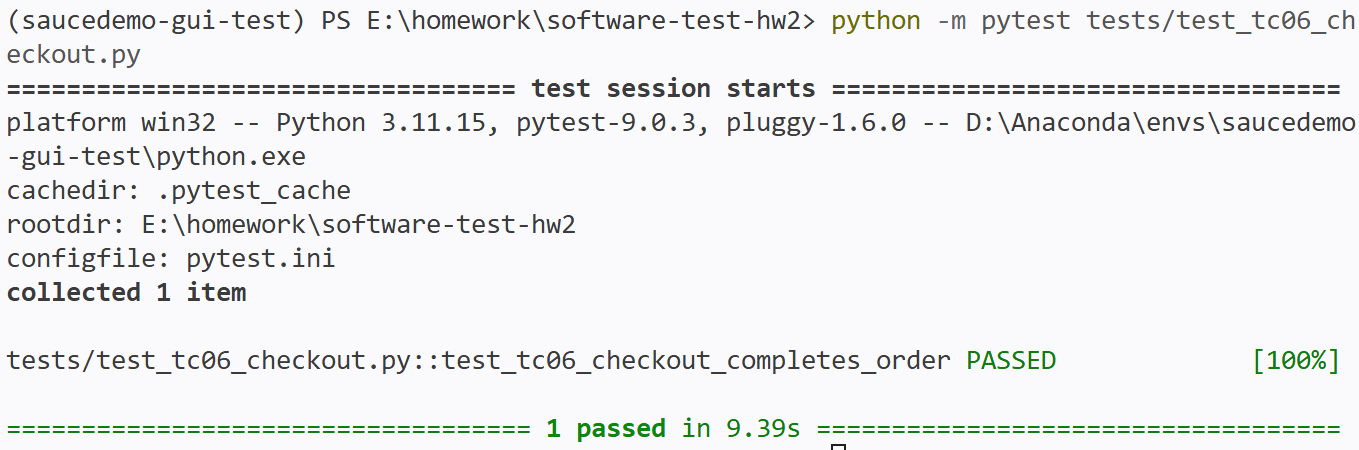
\includegraphics[width=0.92\textwidth]{Figures/TC06_result.png}
\caption{TC06 结算与订单完成执行结果截图}
\end{figure}

\subsection{TC07 侧边栏导航菜单}

TC07 用于验证商品列表页左侧侧边栏导航菜单的展开、菜单项显示和关闭能力。该用例覆盖侧边栏菜单按钮、菜单关闭按钮以及 All Items、About、Logout、Reset App State 等导航项，是对 SauceDemo 导航类交互元素的补充检查。

\begin{table}[H]
\centering
\caption{TC07 测试结果}
\begin{tabularx}{\textwidth}{>{\bfseries}p{3cm}X}
\toprule
项目 & 内容 \\
\midrule
测试文件 & tests/test\_tc07\_sidebar\_navigation.py \\
前置条件 & 已使用标准账号登录并进入商品列表页。 \\
测试步骤 & 检查侧边栏菜单按钮可见；点击菜单按钮展开侧边栏；检查关闭按钮和导航菜单项；点击关闭按钮关闭侧边栏。 \\
实际检查点 & 菜单按钮可见；侧边栏展开后关闭按钮可见；菜单项依次显示 All Items、About、Logout、Reset App State；点击关闭按钮后侧边栏隐藏。 \\
预期结果 & 商品列表页侧边栏能够正常展开和关闭，导航菜单项能够完整显示。 \\
执行结果 & 通过。 \\
\bottomrule
\end{tabularx}
\end{table}

执行结果表明，SauceDemo 商品列表页的侧边栏导航菜单能够被 Selenium 稳定触发，展开后导航项显示完整，关闭按钮能够正常收起侧边栏，导航类交互元素符合预期。

\begin{figure}[H]
\centering
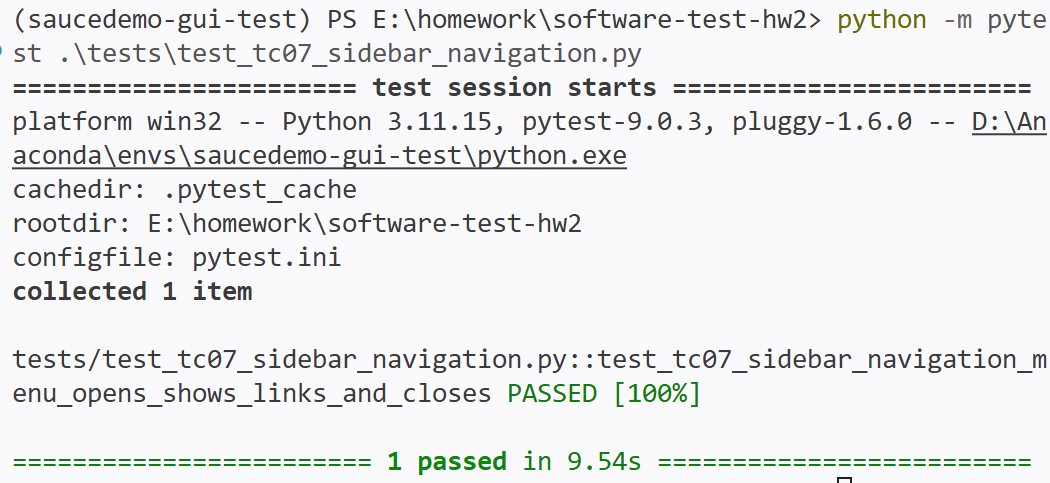
\includegraphics[width=0.92\textwidth]{Figures/TC07_result.png}
\caption{TC07 侧边栏导航菜单执行结果截图}
\end{figure}

\section{移动端 Web UI 测试情况}

移动端 Web UI 测试采用 Appium、UiAutomator2 Driver 和 Android 模拟器中的 Chrome 浏览器执行。测试脚本通过 Appium Server 连接 Android 模拟器，并在模拟器 Chrome 中访问 SauceDemo 网站，从而验证核心购物流程在 Android 移动端浏览器环境下的可用性。

移动端测试执行前，需要先启动 Android 模拟器并确认 adb 能识别设备，再启动 Appium Server 监听 4723 端口。图 \ref{fig:mobile-env-startup} 和图 \ref{fig:mobile-device-ready} 展示了本次移动端测试的环境启动状态。

\begin{figure}[H]
\centering
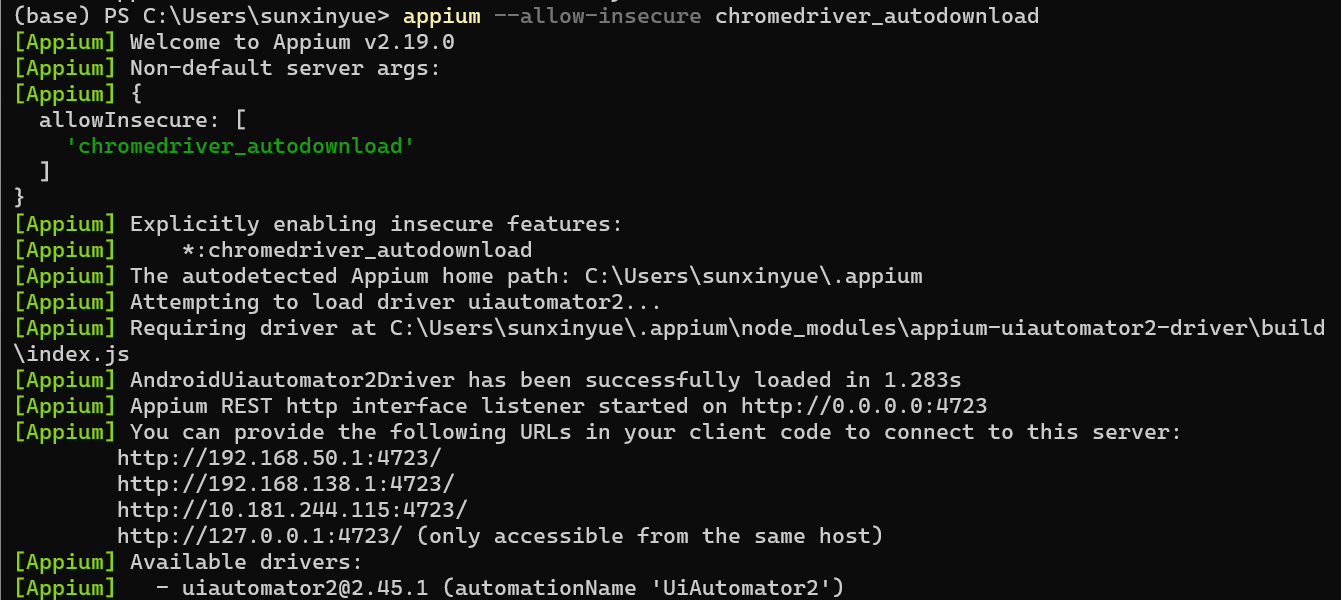
\includegraphics[width=0.92\textwidth]{Figures/appium成功启动截图.png}
\caption{Appium Server 成功启动并监听 4723 端口}
\label{fig:mobile-env-startup}
\end{figure}

\begin{figure}[H]
\centering
\begin{minipage}[c]{0.48\textwidth}
\centering
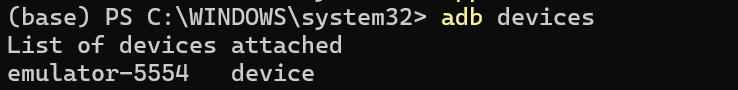
\includegraphics[width=\textwidth]{Figures/adb_devices_命令截图.png}
{\small adb 识别 Android 模拟器}
\end{minipage}
\hfill
\begin{minipage}[c]{0.42\textwidth}
\centering
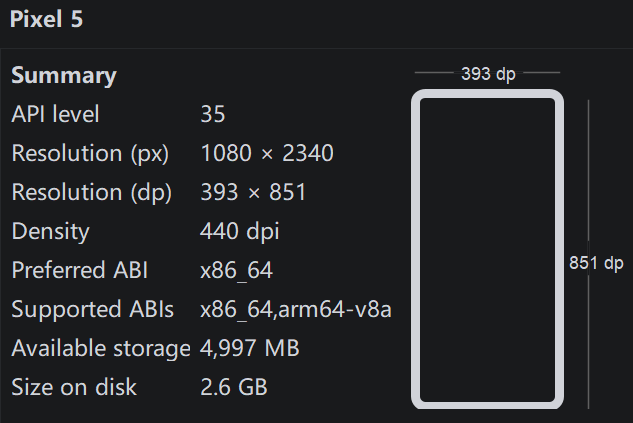
\includegraphics[width=\textwidth]{Figures/安卓手机配置截图.png}
{\small Android 模拟器设备配置}
\end{minipage}
\caption{Android 模拟器连接与设备配置}
\label{fig:mobile-device-ready}
\end{figure}

\begin{table}[H]
\centering
\caption{移动端 Web UI 综合测试结果}
\begin{tabularx}{\textwidth}{>{\bfseries}p{3cm}X}
\toprule
项目 & 内容 \\
\midrule
测试文件 & tests/test\_tc08\_mobile\_appium.py \\
测试环境 & Android Studio 模拟器、Android Chrome、Appium Server、UiAutomator2 Driver、Appium-Python-Client、pytest。 \\
前置条件 & Android 模拟器已启动，adb 能识别设备，Appium Server 使用 appium --allow-insecure chromedriver\_autodownload 启动。 \\
测试范围 & 移动端 Chrome 打开 SauceDemo、登录、商品列表展示、商品排序、页面滚动、商品详情查看、加入购物车、购物车页面检查、结算信息填写、订单确认和订单完成。 \\
实际检查点 & 登录页 username 和 password 输入框可见且可输入；Login 按钮可点击；登录后进入 Products 页面；商品价格排序结果正确；页面可滚动；商品详情页显示 Sauce Labs Backpack 及价格；加入购物车后按钮变为 Remove 且购物车 badge 显示 1；购物车页显示商品名称和数量；结算信息表单可填写；订单确认页和订单完成页均能正常显示。 \\
预期结果 & Android 模拟器 Chrome 环境下，桌面端已覆盖的核心购物流程在移动端也能够正常完成。 \\
执行结果 & 通过。 \\
\bottomrule
\end{tabularx}
\end{table}

执行结果表明，SauceDemo 在 Android 模拟器 Chrome 环境下能够完成从登录、商品浏览、排序、详情查看、加入购物车到结算完成的核心流程。移动端测试没有将 TC01--TC06 完全拆分为多个独立用例重复书写，而是以一个 Appium 综合流程覆盖桌面端主要事务，用于补充证明系统在移动端 Web 浏览器中的关键交互同样可用。

\begin{figure}[H]
\centering
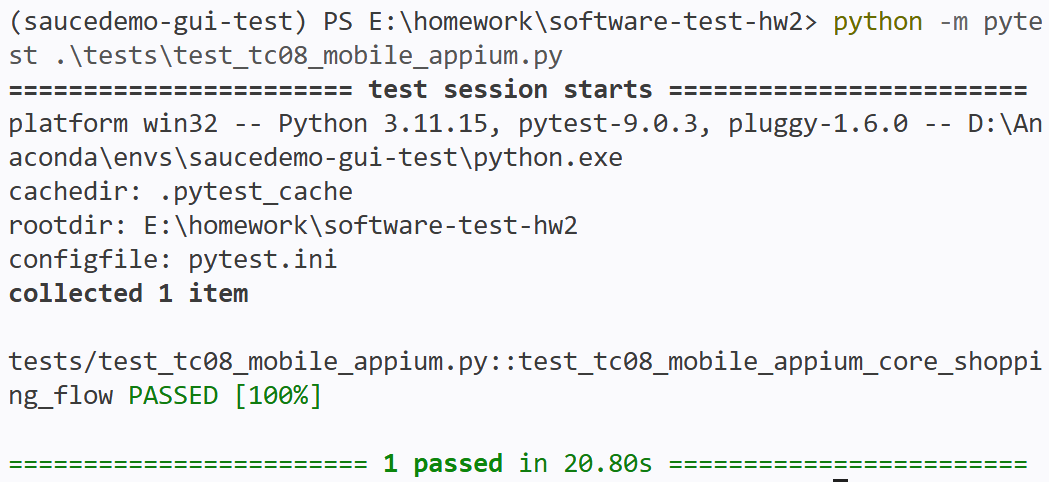
\includegraphics[width=0.92\textwidth]{Figures/TC08_result.png}
\caption{TC08 Appium 移动端 Web UI 综合测试执行结果截图}
\end{figure}

\section{问题与结论}

\subsection{桌面端 Web UI 测试结论}

TC01 和 TC02 均执行通过，验证了标准账号进入商品列表页、商品列表页关键元素显示以及商品排序下拉框的四种排序规则。测试结果表明，SauceDemo 的商品浏览入口和商品排序功能表现正常，未发现影响登录后商品浏览和排序操作的功能异常。

TC03、TC04 和 TC05 均执行通过，验证了商品详情页跳转、商品详情信息展示、添加商品到购物车以及购物车页面商品信息展示等流程。测试结果表明，SauceDemo 的商品详情页能够正确显示商品标题、描述、价格和图片；商品加入购物车后按钮状态与购物车 badge 数量能够正确更新；购物车页面能够正确显示已添加商品的名称、描述、价格、数量以及继续购物和结算入口。成员 B 负责范围内未发现影响商品详情查看和购物车使用的功能异常。

TC06 执行通过，验证了从购物车进入结算信息页、填写结算表单、进入订单确认页并完成订单的完整流程。测试结果表明，SauceDemo 的结算表单输入、订单确认和订单完成提示均符合预期，未发现影响结算与订单完成流程的功能异常。

TC07 执行通过，验证了商品列表页侧边栏导航菜单的展开、导航项显示和关闭流程。测试结果表明，SauceDemo 的侧边栏导航控件能够正常响应用户操作，未发现影响导航菜单使用的功能异常。

综上，桌面端 Web UI 测试覆盖了从登录、商品浏览、排序、详情查看、加入购物车、购物车检查、结算完成到侧边栏导航的主要业务路径。TC01--TC07 均执行通过，未发现影响桌面端核心购物流程和导航交互的功能异常。

\subsection{移动端 Web UI 测试结论}

TC08 移动端 Web UI 综合测试执行通过。测试通过 Appium 控制 Android 模拟器中的 Chrome 浏览器完成核心购物流程，验证了登录输入、按钮触控点击、页面滚动、商品排序、商品详情跳转、购物车状态更新、结算表单填写和订单完成等关键操作。测试结果表明，SauceDemo 的核心业务流程在移动端浏览器环境下也能够正常运行。

移动端测试采用 Android 模拟器中的 Chrome 浏览器执行。测试结果说明，在 Appium 移动端 Web UI 环境下，SauceDemo 的核心购物流程能够完成，移动端页面滚动、触控点击和表单输入等关键交互未发现明显异常。

\section{小组成员贡献与比例}

\begin{table}[H]
\centering
\caption{小组成员贡献与比例}
\begin{tabularx}{\textwidth}{>{\raggedright\arraybackslash}p{2.4cm}Y>{\raggedright\arraybackslash}p{2.2cm}}
\toprule
成员 & 主要贡献 & 贡献比例 \\
\midrule
桂舒芸 & 测试计划编写；登录后商品浏览流程与商品排序相关测试；测试报告对应部分整理。 & 33.3\% \\
石欣睿 & 商品详情、添加商品到购物车、购物车页面检查相关测试与报告内容。 & 33.3\% \\
孙昕玥 & 结算与订单完成、侧边栏导航菜单、Appium 移动端 Web UI 综合验证相关测试与报告内容。 & 33.3\% \\
\bottomrule
\end{tabularx}
\end{table}

\end{document}
